\documentclass[tikz,border=8pt]{standalone}
\usepackage[scaled=0.95]{helvet}
\renewcommand{\familydefault}{\sfdefault}
\usepackage[europeanresistors,americanvoltages]{circuitikz}
\definecolor{TEJNavy}{HTML}{1E2B55}
\definecolor{TEJBlue}{HTML}{1769AA}
\begin{document}
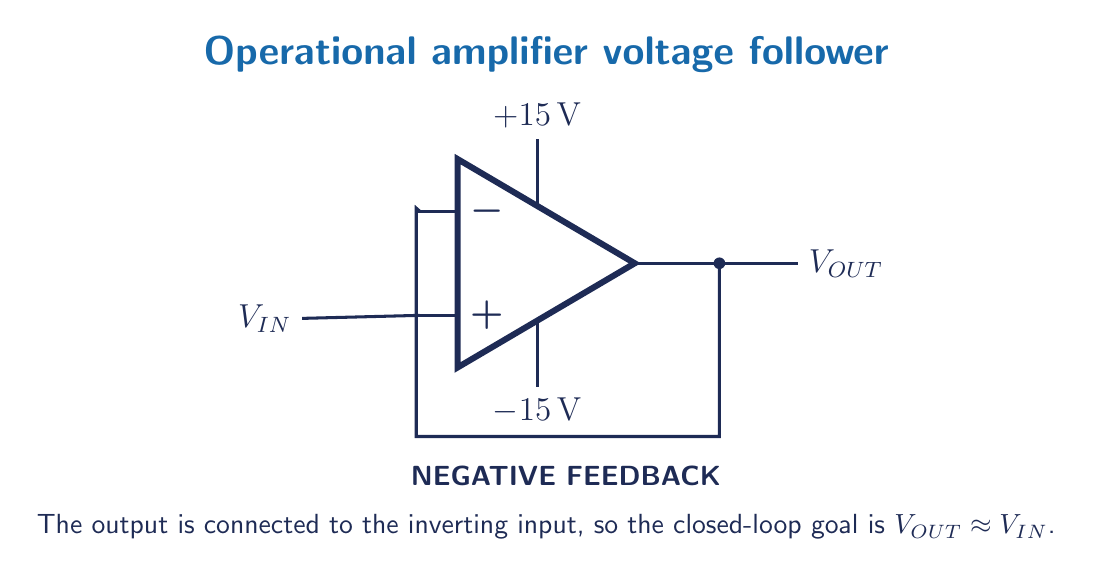
\begin{tikzpicture}[line width=1.1pt,draw=TEJNavy,text=TEJNavy,font=\sffamily]
  \node[font=\bfseries\Large,text=TEJBlue] at (4.0,5.0)
    {Operational amplifier voltage follower};
  \node[op amp,scale=1.35] (A) at (4.0,2.35) {};
  \draw (A.up) -- ++(0,0.85) node[above,font=\large] {$+15\,\mathrm{V}$};
  \draw (A.down) -- ++(0,-0.85) node[below,font=\large] {$-15\,\mathrm{V}$};
  \draw (A.+) -- (0.9,1.65) node[left,font=\large] {$V_{IN}$};
  \draw (A.out) -- (7.2,2.35) node[right,font=\large] {$V_{OUT}$};
  \fill[TEJNavy] (6.2,2.35) circle (2.1pt);
  \draw (6.2,2.35) -- (6.2,0.15) -- (2.35,0.15) -- (2.35,3.05) -- (A.-);
  \node[font=\bfseries] at (4.25,-0.35) {NEGATIVE FEEDBACK};
  \node[align=center] at (4.0,-1.0)
    {The output is connected to the inverting input, so the closed-loop goal is $V_{OUT}\approx V_{IN}$.};
\end{tikzpicture}
\end{document}
